In the previous Chapter we have see how to prepare input for our software. Now we will focus on the proper process conversion. How we will see here, for the conversion we have a \textbf{pipeline of transformations} which progressively refines the results. Firstly we will give an overall overview of the pipeline, then we will see in detail each step.

\section{The conversion pipeline}\label{sec33:Pipeline}

We have already seen in Chapter~\ref{sec31:Grid}, in the conversion process we divide our input into \textit{blocks} which are manipulated in parallel. In particular, we execute several transformations for each block that progressively refine the result. As a consequence we can see that from an architectural point of view \texttt{ImagesToLARModel} is an application based on the pattern \textbf{pipes and filters}, where each conversion step represent a filter whose output is the input for the next one. Actually we have the following steps:
\begin{itemize}
 \item \textbf{Pixel to voxels transformations}
 \item \textbf{Boundaries merge}
 \item \textbf{Block merge}
 \item \textbf{Smoothing}
 \item \textbf{Final model creation}
\end{itemize}

Each step works on a block of the model, so the pseudocode for the definition of a step is the following:

\begin{pseudo}[caption={Single step of the conversion pipeline}, label={lst:stepInvocation}]
begin
  $beginImageStack = 0$
  $endImage = beginImageStack$
  for $zBlock$ from $0$ to $image\; depth / blockDz - 1$:
    $startImage = endImage$
    $endImage = startImage + blockDz$
    for $xBlock$ from $0$ to $image\; width / blockDx - 1$:
      for $yBlock$ from $0$ to $image\; height / blockDy - 1$:
        parallel execute $stepFunction$ on $b=(xBlock,yBlock,zBlock)$
end       
\end{pseudo}

How we can see from the pseudocode, for the implementation of a step, the user have to give the sizes of the block

\section{Converting pixels to voxels}\label{sec33:PixelsToVoxels}

Now we can see the first step of the conversion pipeline: \textbf{conversion from pixels to voxels}. First of all, we need to load only the binary data of the image stack corresponding to the current block obtaining a cuboid geometry of the block. At this point, we can transform the binary matrix into an array. In Figure~\ref{fig:linearizedMatrix} there are two examples showing how this transformation works.

\begin{figure}[htb] %  figure placement: here, top, bottom
   \centering
    \begin{math}
    \begin{pmatrix}
    0^{0} & 0^{2}\\
    0^{1} & 0^{3}
    \end{pmatrix}   
    \begin{pmatrix}
    1^{4} & 0^{6}\\
    1^{5} & 1^{7}
    \end{pmatrix}
    \xrightarrow{}
    \begin{array}{c c c c c c c c}
      0^{0} & 0^{1} & 0^{2} & 0^{3} & 1^{4} & 1^{5} & 0^{6} & 1^{7}
    \end{array}
    $ $    
    \begin{pmatrix}
    0^{0} & 0^{2}\\
    0^{1} & 0^{3}
    \end{pmatrix}
   \begin{pmatrix}
    0^{4} & 1^{6}\\
    1^{5} & 1^{7}
    \end{pmatrix}
    \xrightarrow{}
    \begin{array}{c c c c c c c c}
      0^{0} & 0^{1} & 0^{2} & 0^{3} & 0^{4}  & 1^{5} & 1^{6} & 1^{7}
    \end{array}
    \end{math}
   \hfill
   \caption[Transformation of a matrix resulting from a $2\times 2\times 2$ grid into an array]{Transformation of a matrix resulting from a $2\times 2\times 2$ grid into an array (with cells indexes) (a) First example (b) Second example}
   \label{fig:linearizedMatrix}
\end{figure}

We have already seen that the input for this step consists in binary images which will contain only $0x00$ and $0xff$ values. Obviously we are only interested in non-empty values, so what we have to do now is to iterate on data and get only indices of the array where the value is $0xff$. Consequently, we have obtained a set of pixels that belongs to the model. If we want a real three-dimensional representation, we only have to map a pixel to a voxel transforming flat squares into cube geometries.\\

So far we have obtained a list of cuboidal cells inside a block; however in our representations we want only \textbf{boundary cells}, so we have to find them. How we have seen in Chapter~\ref{sec21:topologicalOperators} it is simple to compute the boundaries using LAR. So at this point we have to convert the list of cells into a LAR model. This is possible by creating a basis for a cell complex (formed by cuboids into a grid of the same size of the image grid with integer coordinates that vary from $(0,0,0)$ to $(blockDx, blockDy, blockDz)$) and saving only cubes whose indices are the same contained in the list we have computed earlier. Final boundary computation can be done computing a \textbf{boundary matrix} for the block of sizes $(blockDx, blockDy, blockDz)$ and, as it depends only on those dimensions, it can be saved somewhere and reused with other models.\\

All this process is \textbf{embarrassingly parallel}, which means that every block can be processed independently of the others.

\begin{figure}[htb] %  figure placement: here, top, bottom
   \centering
   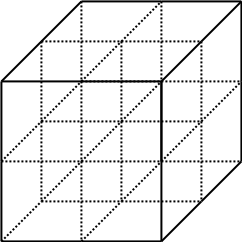
\includegraphics[width=0.25\linewidth]{images/larbasis.png}\hfill
   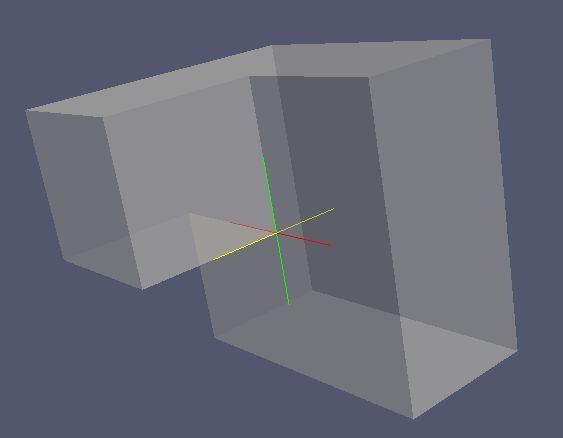
\includegraphics[width=0.30\linewidth]{images/sampleBlock1.png}\hfill
   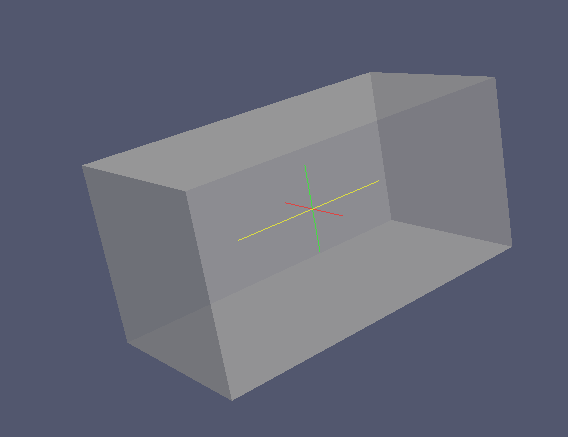
\includegraphics[width=0.30\linewidth]{images/sampleBlock2.png}
   \caption[Sample models of $2 \times 2 \times 2$ blocks]{Sample models of $2 \times 2 \times 2$ blocks. (a) Basis for a $2 \times 2 \times 2$ block. (b) and (c) Representations of sample geometries obtained from the previous basis}
   \label{fig:sampleBlocks}
\end{figure}

\section{Merging boundaries}\label{sec33:Boundaries}

At the end of the previous step, we have obtained at most $\displaystyle\frac{image-width}{blockDx} \times \displaystyle\frac{image-height}{blockDy} \times \displaystyle\frac{image-depth}{blockDz}$ blocks (some of them could be empty). However because of every single block is processed independently of the other we still have boundaries between them. In fact, the boundary operator works only on a single block so we have to \textit{manually remove faces between blocks}. A simple procedure is explained in the following pseudocode and in Figure~\ref{fig:boundaryMergeIteration}:

\begin{pseudo}[caption={Removal of internal boundaries}, label={lst:boundaryRemoval}]
begin
  foreach block $b$:
    $rb$ = next block on the right
    $tb$ = next block on the top
    $fb$ = next block on the front
    $merge$ right boundary of $b$ with left boundary of $rb$
    $merge$ top boundary of $b$ with bottom boundary of $tb$
    $merge$ front boundary of $b$ with back boundary of $fb$
end
\end{pseudo}

\begin{figure}[htb] %  figure placement: here, top, bottom
   \centering
   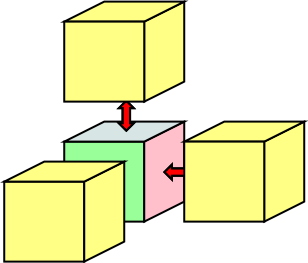
\includegraphics[width=0.30\linewidth]{images/BoundaryMergeIteration.png}
   \caption[Merging of boundary faces]{Merging of boundary faces. For a single block we need adjacent blocks on the right, top and front}
   \label{fig:boundaryMergeIteration}
\end{figure}

How we can see from the pseudocode, the first thing we will need is to recognize boundaries from the interior of a block. In fact, we can decompose a single block into seven parts (listed in Figure~\ref{fig:boundaries}) observing the coordinates of every face.

\begin{figure}[htb] %  figure placement: here, top, bottom
   \centering
   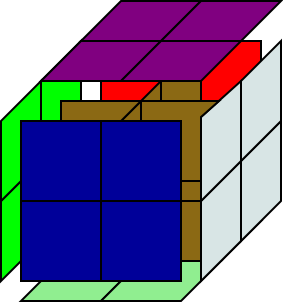
\includegraphics[width=0.25\linewidth]{images/boundaries.png}
   \caption[Decomposition of a LAR model into seven parts]{Decomposition of a LAR model into seven parts: the inside model (brown), the left boundary (green), the right boundary (light blue), the top boundary (purple), the bottom boundary (light green), the front boundary(blue), the back boundary (red)}
   \label{fig:boundaries}
\end{figure}

Now we can focus on the merge procedure. First of all we need to remove double vertices from models. To achieve this goal, we need to iterate on the vertices array and find and remove them saving the indices of the removed ones at the same time. Then we have to reindex the faces in order to remove links to the removed vertices. At this point, we can find faces with the same coordinates and remove them from both blocks we are merging. In Listing~\ref{lst:mergeBoundary} there is the pseudocode for the procedure we have described here.

\begin{pseudo}[caption={Merging of two boundaries}, label={lst:mergeBoundary}]
begin
  concatenate $V_1$ and $V_2$
  concatenate $FV_1$ and $FV_2$
  remove double vertices from $V_1 + V_2$
  reindex vertices indices in $FV_1 + FV_2$
  remove double faces in $FV_1 + FV_2$
end
\end{pseudo}

\begin{figure}[htb] %  figure placement: here, top, bottom
   \centering
   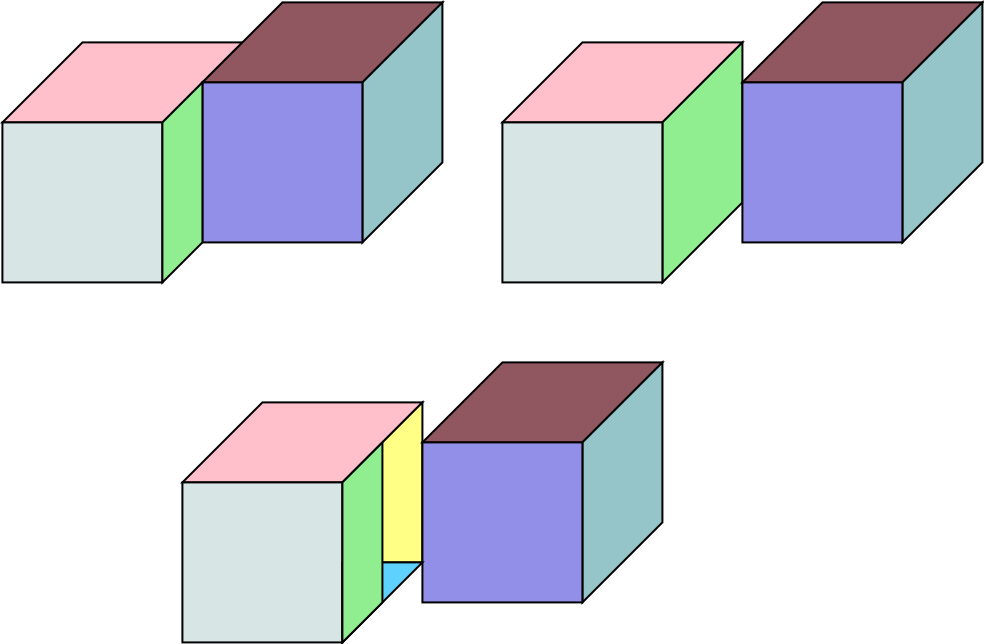
\includegraphics[width=0.40\linewidth]{images/BoundaryMerge.png}
   \caption[Removal of double faces from boundaries]{Removal of double faces from boundaries. (a) Two adjacent blocks (b) The same blocks exploded on x axis (c) Result of the removal on the exploded blocks}
   \label{fig:boundaryMerge}
\end{figure}

\section{Merging blocks}\label{sec33:Blocks}

At the end of the previous step, we have obtained models representing the inner parts of a single block and the boundaries remained after removal of duplicates. Now we are interested in merge all these models into blocks removing duplicated vertices between them, in order to save space and prepare the model to the next step. In fact, the process that produces the models uses adjacent cuboids with duplicated vertices. An example is given in Figure~\ref{fig:duplicates}, where we can see the boundary of a model obtained from a $2 \times 2 \times 2$ grid

\begin{figure}[htb] %  figure placement: here, top, bottom
   \centering
   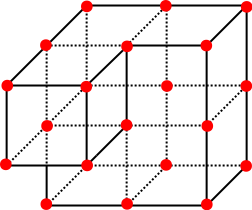
\includegraphics[width=0.25\linewidth]{images/duplicates.png}
   \caption[Sample model with double vertices]{A sample model taken from a $2 \times 2 \times 2$ grid with double vertices between faces in red (remember that we have only the boundaries faces for the model)}
   \label{fig:duplicates}
\end{figure}

As in the previous step we have to concatenate models, remove the repeated coordinates and reindex vertices in faces.

\section{Smoothing}\label{sec33:Smoothing}

At the end of the previous step we have obtained independent blocks without double vertices. However, these blocks are not so good to see, as they have squared edges (remember that they are composed by attached cuboids). As the medical parts usually have rounded edges, now we want to \textbf{smooth} the three-dimensional model.\\

There are many different algorithms for mesh smoothing, the simpler and the one it has been used in the library is \textbf{laplacian smoothing}. Here, for each vertex in a mesh, a new position is chosen according to local information (such as the coordinates of neighbors) and the vertex is moved there. If that mesh is topologically a rectangular grid (so each internal vertex is connected to four neighbors) then this operation produces the \textit{Laplacian} of the mesh.
\begin{figure}[htb] %  figure placement: here, top, bottom
   \centering
   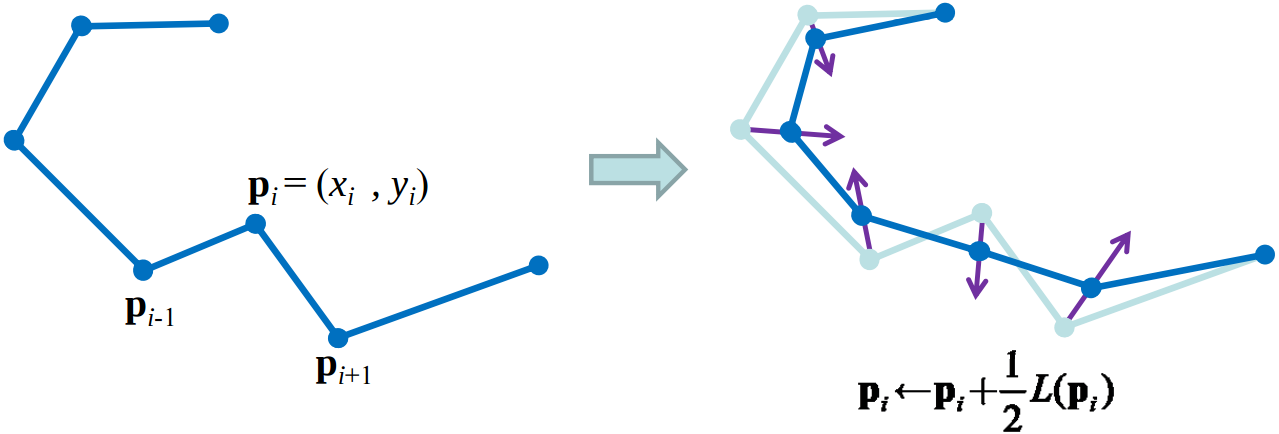
\includegraphics[width=0.60\linewidth]{images/LaplacianSmoothing.png}
   \caption[Laplacian smoothing]{Laplacian smoothing (picture taken from the \textit{Geometry Processing Algorithms} course at Stanford University)}
   \label{fig:laplacianSmoothing}
\end{figure}

As we can see from Figure~\ref{fig:laplacianSmoothing}, with substitution of every vertex position with the mean of the neighbors positions, we can obtain a curve with smoothed edges. This procedure can be repeated many times. This is the pseudocode for laplacian smoothing:

\begin{pseudo}[caption={Laplacian smoothing}, label={lst:laplacianSmoothing}]
begin
  foreach vertex $i$:
    $\bar{x}_{i}= \displaystyle\frac{1}{N} \displaystyle\sum_{j=1}^{N}\bar{x}_j$
end
\end{pseudo}

In that procedure, $N$ is the number of adjacent vertices to vertex $i$, $\bar{x}_{j}$ is the position of the j-th adjacent vertex and $\bar{x}_{i}$ is the new position for $i$. How we can see, computation of adjacent vertices is a very important task. However, using LAR it become simple as we just need to compute the $VV$ relation.\\

Now we can focus on smoothing for our blocks. One great problem that arises from our subdivision is the computation of adjacent vertices on boundaries. In fact we cannot load the entire model into memory due to the enormous sizes. The solution to this problem consists in loading also the near blocks to the one we want to smooth, execute the algorithm and than save only vertices of the block. In Figure~\ref{fig:SmoothingBlocks} there is a graphical explanation for the algorithm while in Listing~\ref{lst:blockSmoothing} there is the pseudocode.

\begin{figure}[htb] %  figure placement: here, top, bottom
   \centering
   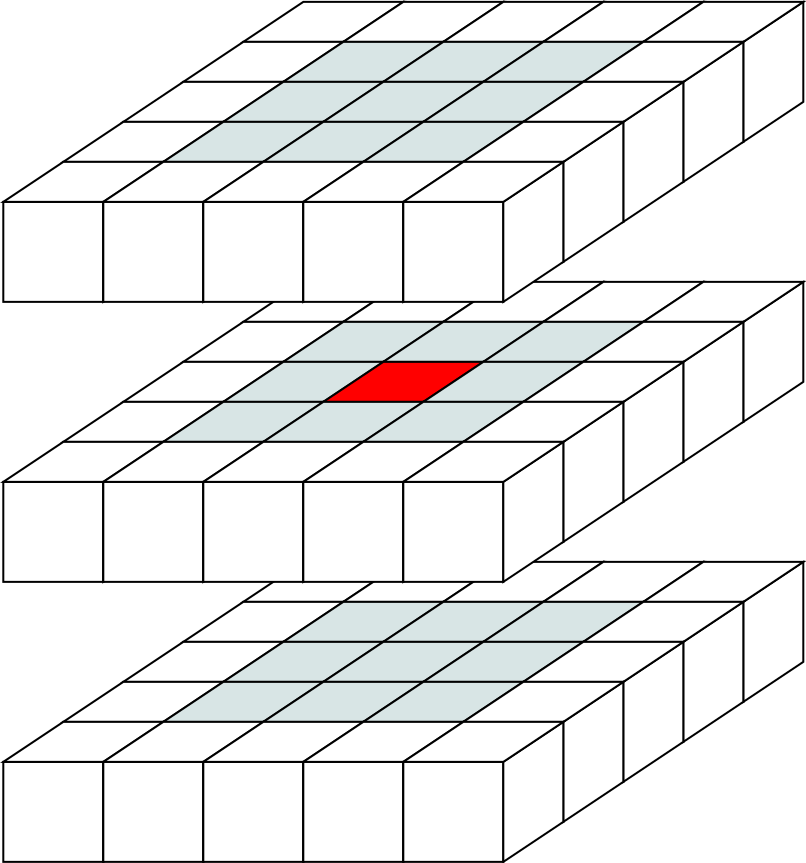
\includegraphics[width=0.30\linewidth]{images/SmoothingBlocks.png}
   \caption[Smoothing of a single block]{Smoothing of a single block. The red block at the center of the figure is the current one, while the other twenty six colored ones are the blocks that will be part of the model which will be smoothed for this iteration}
   \label{fig:SmoothingBlocks}
\end{figure}

\begin{pseudo}[caption={Smoothing of a block}, label={lst:blockSmoothing}]
begin
  foreach block $b$:
    Merge $b$ with its near blocks
    Compute $VV$ relation
    Execute smoothing on the resulting model
    Save new vertices only for $b$
end
\end{pseudo}

\section{Creating the final model}\label{sec33:FinalModel}

At the end of the previous step, we have obtained smoothed blocks. Now, as we want to study the entire model, we have to merge all these blocks in a unique file. The file format chosen is the \textbf{wavefront obj} format, which is simple and widespread. The syntax used is the following:

\begin{itemize}
 \item All vertices are described with their coordinates and written on a single row according to the following syntax:\\ $\texttt{v xCoord yCoord zCoord}$
 \item All faces are described with their vertex index (calculated from their row) according to the following syntax:\\ $\texttt{f vertex1 vertex2 \dots vertexn}$
\end{itemize}

In Figure~\ref{fig:objSample} there is an example of an obj file

\begin{figure}[htb] %  figure placement: here, top, bottom
   \centering
   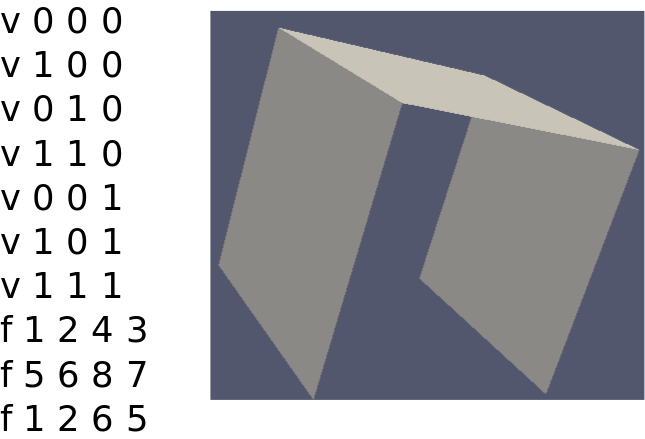
\includegraphics[width=0.40\linewidth]{images/objSample.png}
   \caption{Obj sample file}
   \label{fig:objSample}
\end{figure}

We can see that this kind of representation is very similar to the LAR representation schema, so we just have to read every element of $V$ and $FV$ (in the list of indices format) and write them on disk.\\

At the end of this step, we will have the full model in obj format which can be observed on every three-dimensional viewer.